%
% This document contains the chapter about other transmission lines.
%
% Copyright (C) 2006 Stefan Jahn <stefan@lkcc.org>
%
% Permission is granted to copy, distribute and/or modify this document
% under the terms of the GNU Free Documentation License, Version 1.1
% or any later version published by the Free Software Foundation.
%

\chapter{Other types of transmission lines}
%\addcontentsline{toc}{chapter}{Other types of transmission lines}

\section{Coaxial cable}
%\addcontentsline{toc}{section}{Coaxial cable}

\begin{figure}[ht]
\begin{center}
\psfrag{er}{$\mathrm{\varepsilon_r}$}
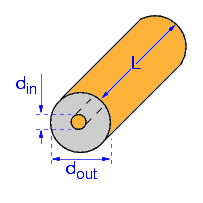
\includegraphics[width=0.35\linewidth]{coax}
\end{center}
\caption{coaxial line}
\label{fig:coax}
\end{figure}
\FloatBarrier

\subsection{Characteristic impedance}
%\addcontentsline{toc}{subsection}{Characteristic impedance}

The characteristic impedance of a coaxial line can be calculated as follows:
\begin{equation}
Z_0 = \dfrac{Z_{F0}}{2\pi\cdot\sqrt{\varepsilon_r}}\cdot\ln{\left(\dfrac{D}{d}\right)}
\end{equation}

\subsection{Losses}
%\addcontentsline{toc}{subsection}{Losses}

Overall losses in a coaxial cable consist of dielectric and conductor
losses.  The dielectric losses compute as follows:
\begin{equation}
\alpha_d = \dfrac{\pi}{c_0}\cdot f\cdot \sqrt{\varepsilon_r} \cdot \tan{\delta}
\end{equation}

The conductor (i.e. ohmic) losses are specified by
\begin{equation}
\alpha_c = \dfrac{1}{2}\cdot \sqrt{\varepsilon_r} \cdot\left(\dfrac{\dfrac{1}{D} + \dfrac{1}{d}}{\ln{\left(\dfrac{D}{d}\right)}}\right)\cdot\dfrac{R_S}{Z_{F0}}
\end{equation}

with $R_S$ denoting the sheet resistance of the conductor material,
i.e. the skin resistance
\begin{equation}
R_S = \sqrt{\pi\cdot f\cdot \mu_r \cdot \mu_o \cdot \rho}
\end{equation}

\subsection{Cutoff frequencies}
%\addcontentsline{toc}{subsection}{Cutoff frequencies}

In normal operation a signal wave passes through the coaxial line as a
TEM wave with no electrical or magnetic field component in the
direction of propagation.  Beyond a certain cutoff frequency
additional (unwanted) higher order modes are excited.
\begin{align}
f_{TE} &\approx \dfrac{c_0}{\pi\cdot\left(D + d\right)}
\;\;\;\;\rightarrow\;\;\;\; \textrm{TE(1,1) mode}\\
f_{TM} &\approx \dfrac{c_0}{2\cdot\left(D - d\right)}
\;\;\;\;\rightarrow\;\;\;\; \textrm{TM(n,1) mode}
\end{align}

\section{Twisted pair}
%\addcontentsline{toc}{section}{Twisted pair}

The twisted pair configurations as shown in fig. \ref{fig:twisted}
provides good low frequency shielding.  Undesired signals tend to be
coupled equally into eachline of the pair.  A differential receiver
will therefore completely cancel the interference.

\begin{figure}[ht]
\begin{center}
\psfrag{er}{$\mathrm{\varepsilon_r}$}
\includegraphics[width=0.3\linewidth]{twisted}
\end{center}
\caption{twisted pair configuration}
\label{fig:twisted}
\end{figure}
\FloatBarrier

According to P. Lefferson \cite{Lefferson} the characteristic
impedance and effective dielectric constant of a twisted pair can be
calculated as follows.
\begin{align}
Z_0 &= \dfrac{Z_{F0}}{\pi\cdot\sqrt{\varepsilon_{r,eff}}}\cdot\textrm{sech}\left(\dfrac{D}{d}\right)\\
\label{eq:TPereff}
\varepsilon_{r,eff} &= \varepsilon_{r,1} + q\cdot\left(\varepsilon_r - \varepsilon_{r,1}\right)
\end{align}

with
\begin{equation}
\label{eq:TPq}
q = 0.25 + 0.0004\cdot \theta^2
\;\;\;\; \textrm{ and } \;\;\;\;
\theta = \cot{\left(T\cdot\pi\cdot D\right)}
\end{equation}

whereas $\theta$ is the pitch angle of the twist; the angle between
the twisted pair's center line and the twist.  It was found to be
optimal for $\theta$ to be between 20\degree and 45\degree.  $T$
denotes the twists per length.  Eq. \eqref{eq:TPq} is valid for film
insulations, for the softer PTFE material it should be modified a
follows.
\begin{equation}
q = 0.25 + 0.001\cdot \theta^2
\end{equation}

Assuming air as dielectric around the wires yields 1's replacing
$\varepsilon_{r,1}$ in eq. \eqref{eq:TPereff}.  The wire's total
length before twisting in terms of the number of turns $N$ is
\begin{equation}
l = N\cdot\pi\cdot D\cdot\sqrt{1 + \dfrac{1}{\tan^2{\theta}}}
\end{equation}
